\documentclass[12pt, titlepage]{article}

\usepackage{amsmath, mathtools}

\usepackage{amsfonts}
\usepackage{amssymb}
\usepackage{graphicx}
\usepackage{colortbl}
\usepackage{xr}
\usepackage{hyperref}
\usepackage{longtable}
\usepackage{xfrac}
\usepackage{tabularx}
\usepackage{float}
\usepackage{siunitx}
\usepackage{booktabs}
\usepackage{multirow}
\usepackage[section]{placeins}
\usepackage{caption}
\usepackage{fullpage}
\usepackage{cite}
\usepackage{breqn}

\input{../../Comments}
%% Common Parts

\newcommand{\progname}{Audio360} % PUT YOUR PROGRAM NAME HERE
\newcommand{\authname}{Team 6, SixSense
\\ Omar Alam
\\ Sathurshan Arulmohan
\\ Nirmal Chaudhari
\\ Kalp Shah
\\ Jay Sharma
} % AUTHOR NAMES                  

\usepackage{hyperref}
    \hypersetup{colorlinks=true, linkcolor=blue, citecolor=blue, filecolor=blue,
                urlcolor=blue, unicode=false}
    \urlstyle{same}
                                


\externaldocument[SRS-]{../../SRS/SRS}

\begin{document}

\title{Hardware Report\\\progname}

\author{\authname}

\date{}

\maketitle

\pagenumbering{roman}

\newpage
\section{Revision History}

\begin{table}[hp]
\caption{Revision History} \label{TblRevisionHistory}
\begin{tabularx}{\textwidth}{llX}
\toprule
\textbf{Date} & \textbf{Developer(s)} & \textbf{Change}\\
\midrule
Dec 21, 2025 & Sathurshan, Omar & Report outline.\\
\bottomrule
\end{tabularx}
\end{table}

\newpage

\tableofcontents

\newpage

\pagenumbering{arabic}

\section{Introduction}
\wss{Explain the prupose of this document. Why it was selected for this project}
\wss{Briefly outline the structure of the document}

\section{Hardware}

\subsection{Hardware Requirements}
\wss{Write down requirements that applied to hardware from SRS.}
\wss{Write down any constraints (budget)}

\subsection{Required Hardware Conponents}
\wss{List what hardware is required based on the requirements from above section.}
\wss{Explain how each hardware acheives each requirements/ why it is needed?}
\wss{microcontroller, microphone, Rokid glasses \cite{RokidGlasses}}

\subsection{Hardware Selection Process}
\wss{Process of selecting hardware to fit requirements and pricing}
\wss{performance, cost, timing of shipment, etc.}
\wss{Aleternative hardware}
\wss{Include links to hardware source}

\subsection{Hardware Specification}
\wss{Include specification table of each hardware.}
\wss{Include links to manufacturing documentation whether online or in this repo}

\subsubsection{STM microcontoller}

\subsubsection{Microphone}
\wss{Go over each pin}

\subsubsection{Rokid AR glasses}

\section{Theory}

This section reviews the theoretical background of hardware and software
integration required for this project. It provides the necessary context to
understand the design decisions made by the team. The information presented in
this section comes from Digikey's documentation \cite{I2S} and the 
STM 32 Reference Manual \cite{STM_REFERENCE_MANUAL}.

\subsection{I2S Communication Protocol}

I2S (Inter-Integrated Circuit Sound) is a serial communication protocol designed
specifically for the transmission of digital audio data between integrated
circuits. It enables synchronous and low-latency audio transfer, making it well
suited for applications involving microphones, speakers, and audio devices where
precise timing and synchronization are required. In systems with multiple
microphones, I2S ensures that all devices sample and transmit data using a
common clock, allowing for accurate time alignment of audio signals.
\newline
\newline
\noindent The protocol uses three primary signal lines:
\begin{itemize}
    \item \textbf{SCK (Serial Clock or Bit Clock)}: Controls the timing of each
        transmitted data bit and synchronizes all connected devices.
    \item \textbf{WS (Word Select or Left/Right Clock)}: Indicates whether the
        data being transmitted corresponds to the left or right audio channel.
    \item \textbf{SD (Serial Data)}: Carries the audio sample data.
\end{itemize}

I2S operates using a controller-peripheral (master-slave) architecture. One
device generates the clock signals (SCK and WS) and is referred to as the
controller, while the remaining devices act as peripherals and transmit or
receive audio data accordingly. In this project, the STM32 microcontroller
functions as the controller, generating both the serial clock and word select
signals. The microphones act as peripherals and transmit audio samples on the
SD line in synchronization with these clocks.

Data transmission occurs on either the rising or falling edge of the serial
clock, depending on the configuration of the devices during initialization.
The WS signal changes state once per audio frame, indicating whether the
transmitted data corresponds to the left or right channel. Each audio sample
is aligned with the WS signal such that one complete word is transmitted per
channel per frame. Figure~\ref{fig:i2s_protocol} illustrates the timing
relationship between SCK, WS, and SD.

\begin{figure}[H]
    \centering
    \includegraphics[width=0.75\linewidth]{i2s_protocol.png}
    \caption{I2S protocol as explained from STM32 reference manual.}
    \label{fig:i2s_protocol}
\end{figure}

Audio samples are commonly 16, 24, or 32 bits in length. In this project,
the microphones output 24 bit samples. Since the STM32 microcontroller store
data in 32-bit registers, the received samples require post-processing to
handle proper alignment and padding. This involves shifting the received data.
The microphones transmit data most significant bit (MSB) first, as defined by
the I2S standard. This transmission order is independent of the
microcontroller's internal endianness. Therefore, software must correctly
reconstruct the sample values from the received byte stream. Figure
\ref{fig:i2s_protocol} shows how I2S data is received and stored on the
microcontoller.

\begin{figure}[H]
    \centering
    \includegraphics[width=0.75\linewidth]{i2s_data_transfer.png}
    \caption{I2S data transfer.}
    \label{fig:i2s_data_transfer}
\end{figure}

Figure~\ref{fig:mic} shows the I2S microphone used in this project.
The device provides dedicated pins for the clock (SCK), word select (WS), and
serial data (SD) connections, allowing direct interfacing with the
microcontroller's I2S peripheral.

\begin{figure}[H]
    \centering
    \includegraphics[width=0.4\linewidth]{../../Images/mic.jpg}
    \caption{I2S microphone.}
    \label{fig:mic}
\end{figure}

\subsection{Micophone Synchronization} \label{sec:mic_sync}

Microphone synchronization ensures that audio samples captured from multiple
microphones correspond to the same point in time. This simultaneity is critical
for this project because direction-of-arrival (DoA) estimation relies on
accurately measuring the time differences at which a sound reaches each
microphone (\hyperref[SRS-FR1_2]{FR1.2}).

The microphones communicate using the I2S protocol and are synchronized through
a shared clock. The microcontroller operates as the I2S master and generates
the serial clock (SCK) and word select (WS) signals, while all microphones
operate as slaves. These signals are distributed to each microphone, ensuring
that all devices sample audio simultaneously and remain phase-aligned.
Using a common clock eliminates inter-channel clock drift and minimizes
sampling jitter between microphones. Furthermore, a shared WS signal
guarantees that samples from corresponding channels are aligned consistently in
software buffers for subsequent processing.

Figure~\ref{fig:mic_wiring} illustrates the microphone wiring.
The orange wire represents the SCK signal and the green wire represents the
WS signal. Both signals are common to all microphones in the array.

\begin{figure}[H]
    \centering
    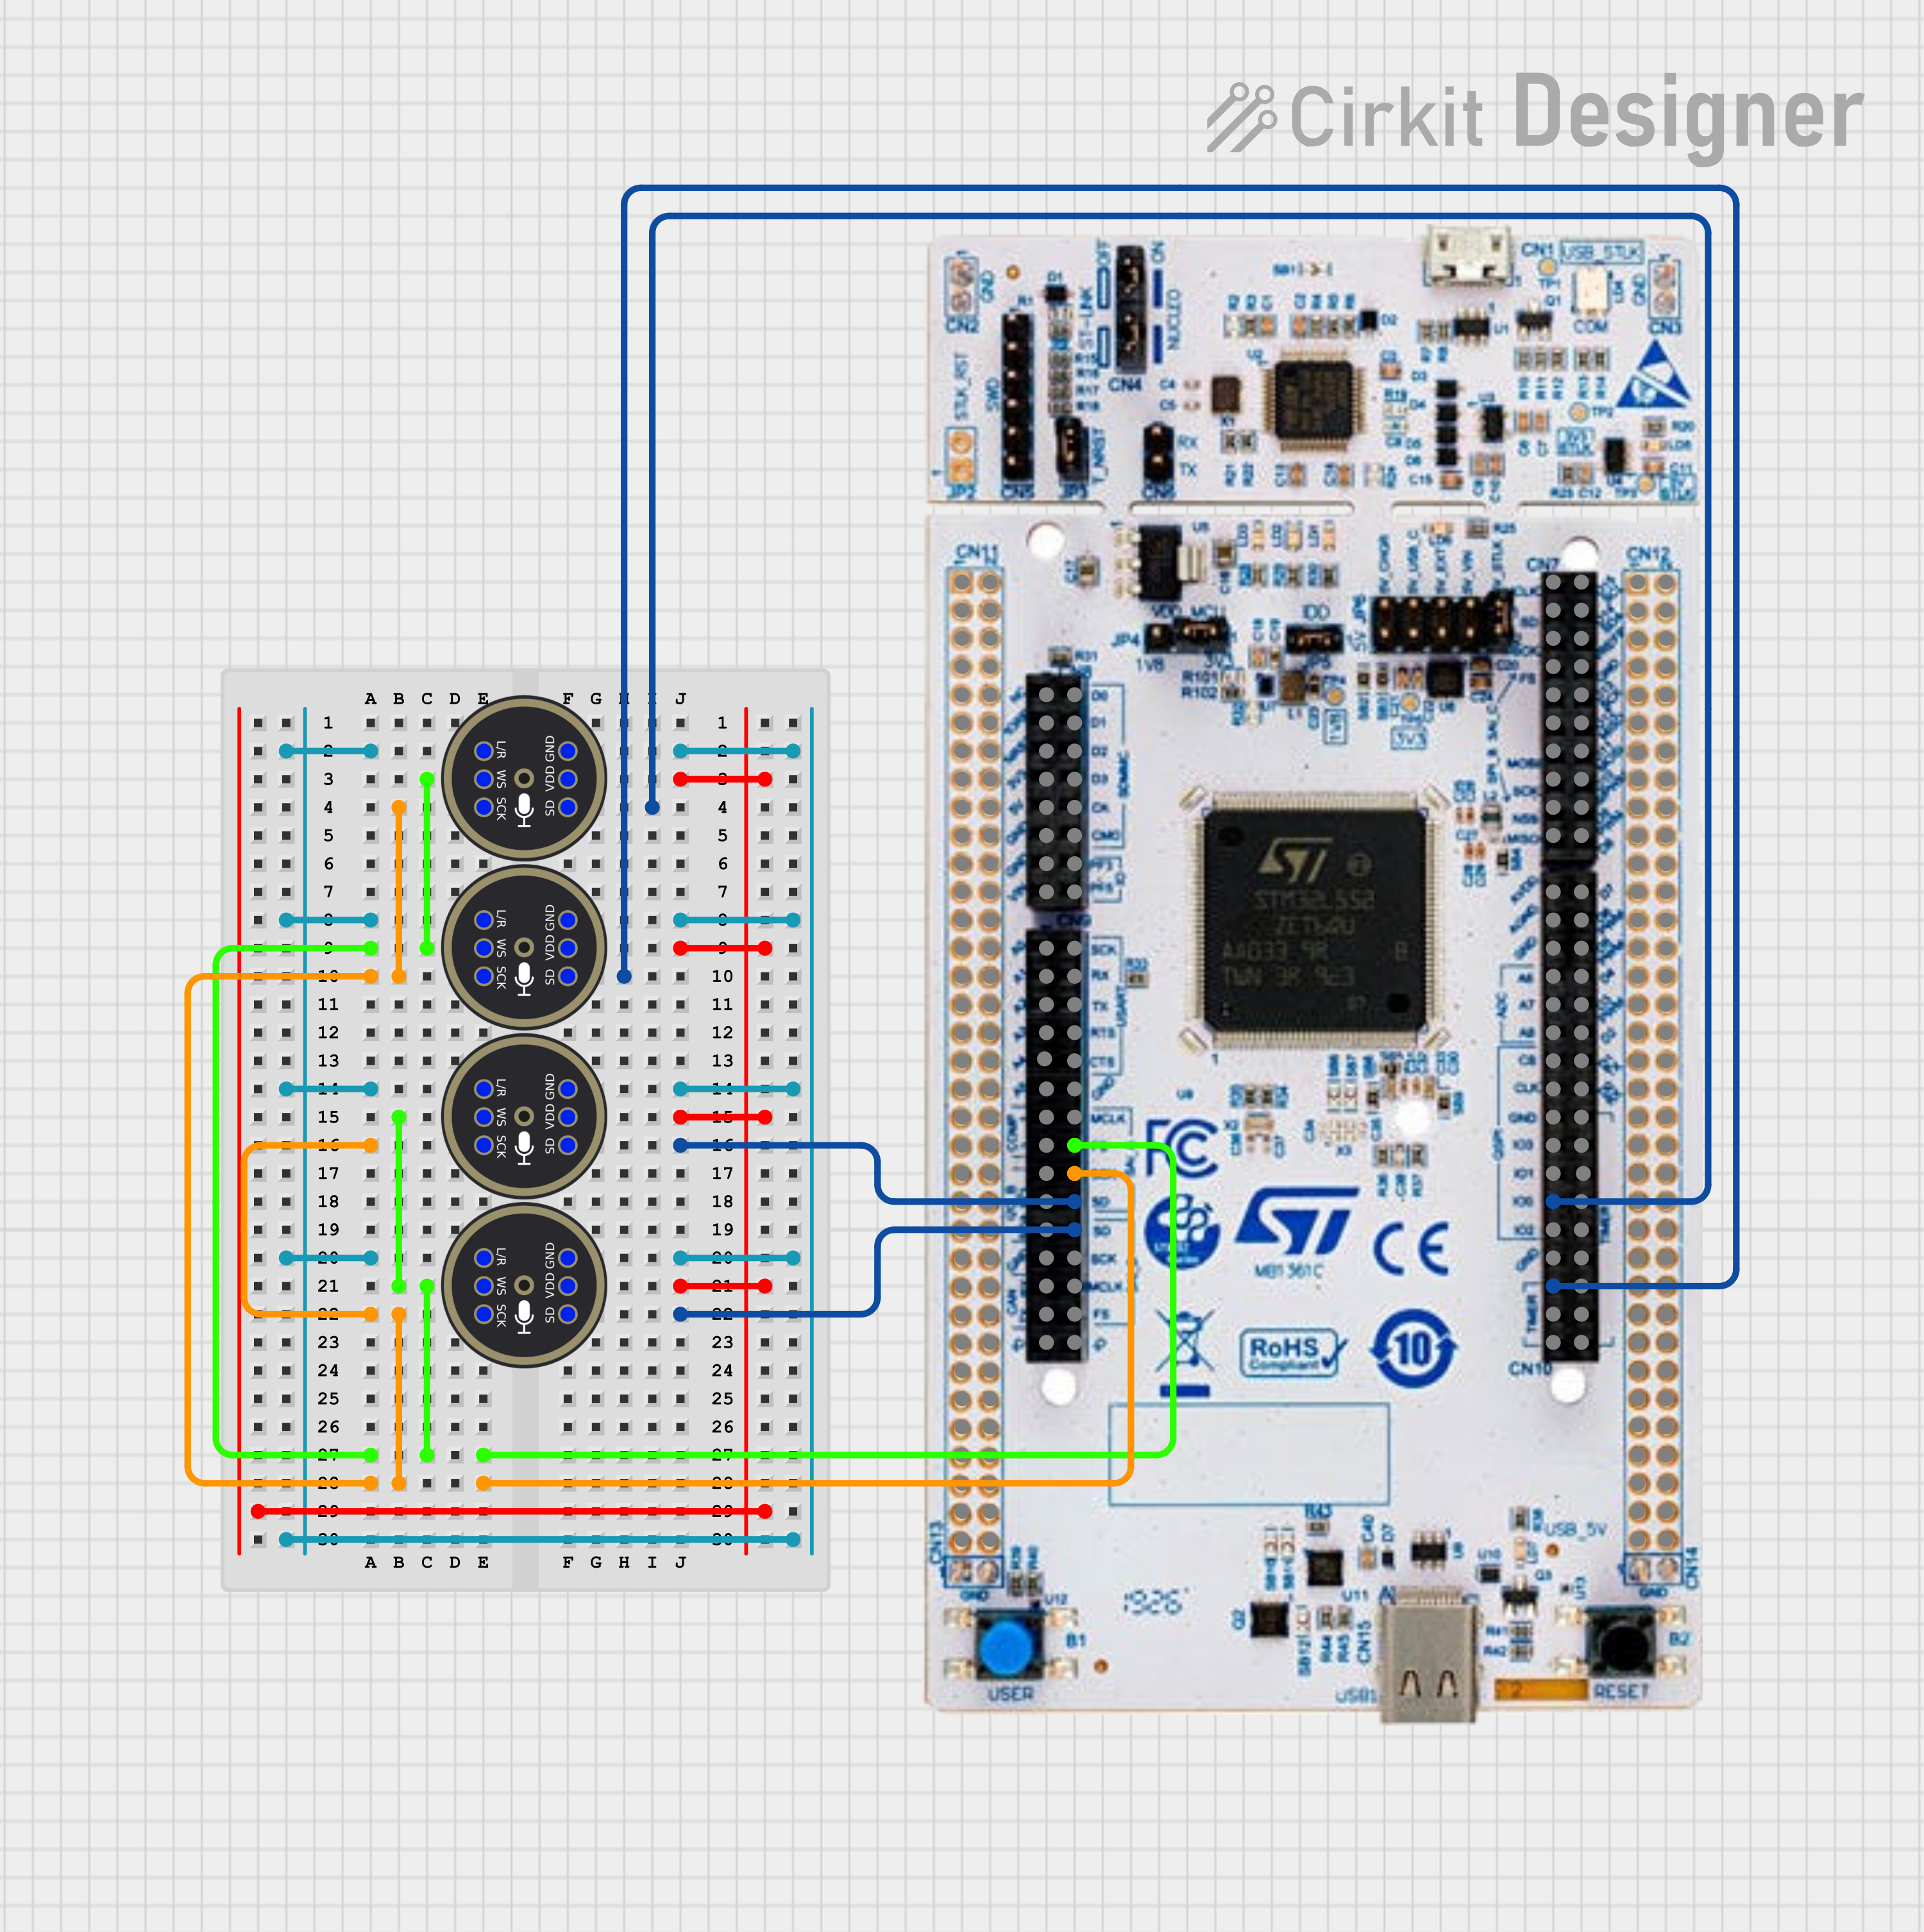
\includegraphics[width=0.75\linewidth]{wiring/microphone_array.png}
    \caption{Microphone wiring. Note that this diagram does not represent the
        exact microphone array position. The purpose is to illustrate the
        wiring.}
    \label{fig:mic_wiring}
\end{figure}

\section{Hardware Integration}

\subsection{Wiring}

Figure~\ref{fig:mic_wiring} illustrates the microphone array wiring
configuration. As described in Section~\ref{sec:mic_sync}, the serial clock
(SCK) and word select (WS) signals are shared among all microphones to achieve
synchronized sampling. The left/right (L/R) channel signal is identical for all
microphones to ensure that each device stores data within the same channel
frame. In this project, all microphones are storing to left channel
(arbitrarily chosen).

Each microphone has an independent data line (blue wire) that transmits
digitized audio data to the microcontroller. These data lines are connected to
the microcontroller input pins PE6, PE3, PD11, and PA0. Power and ground
connections are supplied to each microphone to ensure proper operation.

A micro-USB cable is used to transmit data from the microcontroller to the
smart glasses. Data is communicated via the USB transmit (TX) interface.
Therefore, the connector on the receiving end may vary, provided that the
connected device operates as a USB host.

\subsection{Verification}

Throughout the development of the capstone project, not all hardware components
were available immediately. The smart glasses were expected to arrive
approximately four months into the project, and the printed circuit board (PCB)
for the glasses could not be designed until the wiring of all hardware
components had been finalized. 

As a result, hardware integration was divided into multiple development phases,
allowing the system design to evolve iteratively while software development and
testing proceeded in parallel. This section presents a chronological overview of
the hardware integration evolution process.

\subsubsection{Phase 1: Microcontroller Bring-Up}
In this phase, the team focused on establishing a development environment for
the microcontroller. The primary objective was to build and execute a simple
\textit{Hello World} application to verify correct compilation, flashing, and
execution on the target hardware. This phase enabled familiarity with the
microcontroller toolchain and development workflow.

USB serial communication was then implemented to transmit log data from the
microcontroller to a debugging laptop. This capability was essential, as it
provided the only means of observing internal system behavior during early
development using the CLion debugger.

\subsubsection{Phase 2: Microphone Integration}

Microphones became available in mid October and were subsequently wired to the
microcontroller. Initial development began with a single microphone to verify
configuration and data acquisition before scaling to a
four microphone synchronized array.

To evaluate microphone performance, an SD card module was added to the
microcontroller, and captured audio data were stored as \texttt{.wav} files for
offline playback and verification. In parallel, the serial communication
infrastructure developed in Phase~1 was reused to stream audio data to a host
computer. A Python script was implemented to visualize microphone frequency
responses in real time and provide live audio playback.

These tools enabled rapid verification of microphone functionality and
facilitated detection of wiring and soldering errors. The resulting microphone
array configuration is illustrated in Figure~\ref{fig:mic_wiring}.

\subsubsection{Phase 3: Glasses Integration and System Validation}

In Phase~3, the microphone array was reconfigured to match the physical
dimensions of the smart glasses, figure
\ref{fig:phase3_hardware}. This allowed direction-of-arrival (DoA)
estimation and sound classification algorithms to be evaluated directly on the
microcontroller which was representative of the final product.

During this phase, the smart glasses hardware arrived, enabling the development
of a custom communication protocol between the microcontroller and the glasses.
With these components integrated, the system achieved full end-to-end
functionality.

\begin{figure}[H]
    \centering
    \includegraphics[width=0.75\linewidth]{phase3_hardware.jpg}
    \caption{Hardware configuration during Phase 3.}
    \label{fig:phase3_hardware}
\end{figure}

\subsubsection{Phase 4: PCB Implementation}

In the final phase, the wiring was transitioned from a breadboard based
prototype to a custom PCB. This reduced the risk of loose connections, and
enhanced the overall appearance and robustness of the final product.


\section{Software-Hardware Integration}

This section describes how the software was designed in accordance with the
hardware architecture. As software engineering students, it was essential to
account for the hardware's limitations and capabilities, as these constraints
directly influenced the overall software design and implementation decisions.

\subsection{Hardware Abstraction Layer}

At the beginning of the project, there was significant uncertainty regarding
the availability and suitability of the hardware. It was unclear whether the
team would have access to smart glasses for data visualization or a
microcontroller capable of processing audio data in real time. To mitigate
these risks, contingency plans were developed. For example, the smart glasses
could be replaced with a monitor to display user output, or audio data could be
collected on the microcontroller and streamed to a laptop with sufficient
computational resources to execute the \progname{} features.

Given this uncertainty, the decision was made to abstract the hardware from the
software implementation by introducing a hardware abstraction layer (HAL),
figure \ref{fig:system_layer}.
This layer provides a uniform software interface that is independent of the
underlying hardware. Only the hardware specific interfacing code must be
modified if components are replaced.

The primary benefit of this design choice is improved portability and reduced
dependency on specific hardware platforms, thereby lowering project risk in the
context of a software engineering capstone. However, this approach introduces
additional complexity in both implementation and maintenance of the generalized
abstraction layer.

The hardware abstraction layer is implemented in $src/hardware\_interface$
folder. STM32 interfacing code is located in $src/lib/STM32CubeF7$ folder.

\begin{figure}[H]
    \centering
    \includegraphics[width=0.4\linewidth]{sys_layer.png}
    \caption{System layer diagram.}
    \label{fig:system_layer}
\end{figure}

\subsection{Software Considerations}

Hardware constraints significantly influenced software design decisions at the
implementation level. In particular, the microcontroller provides approximately
500 KB of usable RAM, which is insufficient for computationally intensive tasks.
As a result, the software was designed to minimize memory usage by reusing
objects by employing references instead of creating unnecessary copies.

With this constraint, all algorithms were required to be lightweight and
memory-efficient. This is the primary reason for the team not implementing
a machine learning model for audio classification or direction of arrival
estimation, as there was insufficient memory to store and execute such models.
Additionally, limited RAM capacity restricted the number of audio samples that
could be processed simultaneously. While a larger number of samples generally
improves signal quality and analysis accuracy, memory limitations constrained
the system to approximately 2000 samples per microphone
(about 125~ms of audio data).

Given the potential for hardware-related failures, the software was designed
with error detection and recovery mechanisms if possible. All operations
susceptible to failure, including memory allocation, configuration, and
hardware initialization, are explicitly checked, and appropriate error codes are
returned and handled accordingly. Without these safeguards, the system would
default to an infinite loop of doing nothing, which degrades user experience.
Incorporating structured error handling also enables more efficient debugging
of system faults during development.

\newpage 

\bibliographystyle{IEEEtran}
\bibliography{../../../refs/References}

\end{document}